\section{Mehrdimensionale Wahrscheinlichkeitsrechnung}

\subsection{Formeln}

\subsubsection{Kovarianz, Korrelation}
\begin{equation*}
    Cov[X,Y]=E[(X-E[X])(Y-E[Y])]
\end{equation*}

\begin{equation*}
    Cov[X,Y]=E[XY]-E[X]E[Y]
\end{equation*}

\begin{equation*}
    Cov[X,Y]=Cov[Y,X] \text{ und } Cov[X,X]=Var[X]
\end{equation*}

\begin{equation*}
    Cor[X,Y]=\frac{Cov[X,Y]}{\sqrt{Var(X)Var(Y)}} \rightarrow [-1;+1]
\end{equation*}

\subsubsection{Linearkombinationen}
\begin{equation*}
    E[aX+bY]=aE[X]+bE[Y]
\end{equation*}

\begin{equation*}
    Var[ax+bX]=a^2Var[X]+b^2Var[Y]+2abCov[X,Y]
\end{equation*}

\subsubsection{Mengen}

\begin{figure}[ht]
    \centering
    \begin{minipage}{.5\textwidth}
      \centering
      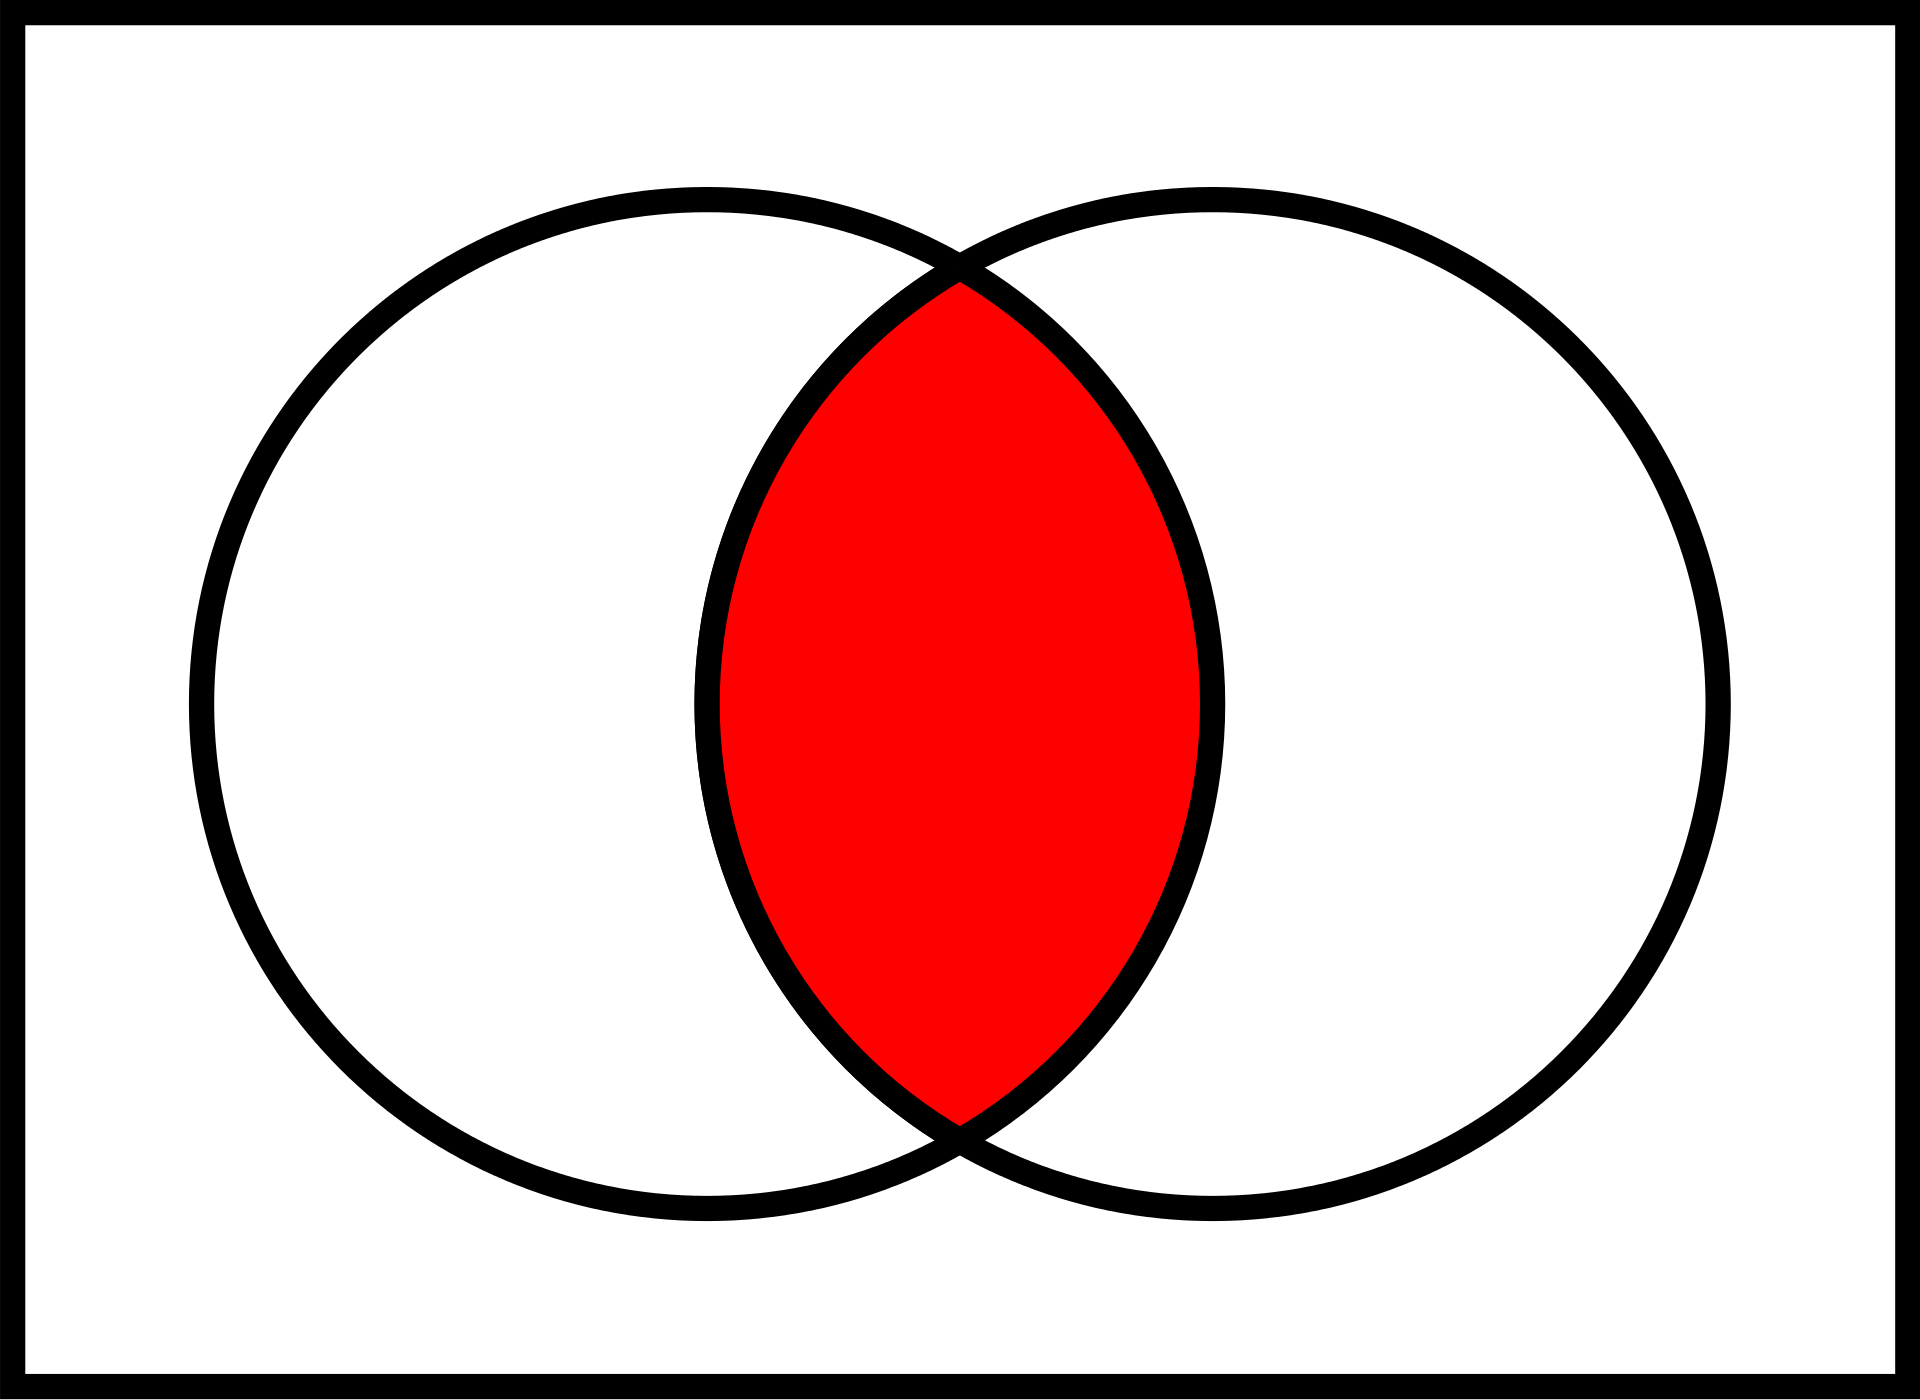
\includegraphics[width=.4\linewidth]{mehrdimWktrechnung/Venn0001.svg.png}
      \captionof*{figure}{Schnittmenge \(A\cap B\)}
      \label{fig:schnittmenge}
    \end{minipage}%
    \begin{minipage}{.5\textwidth}
      \centering
      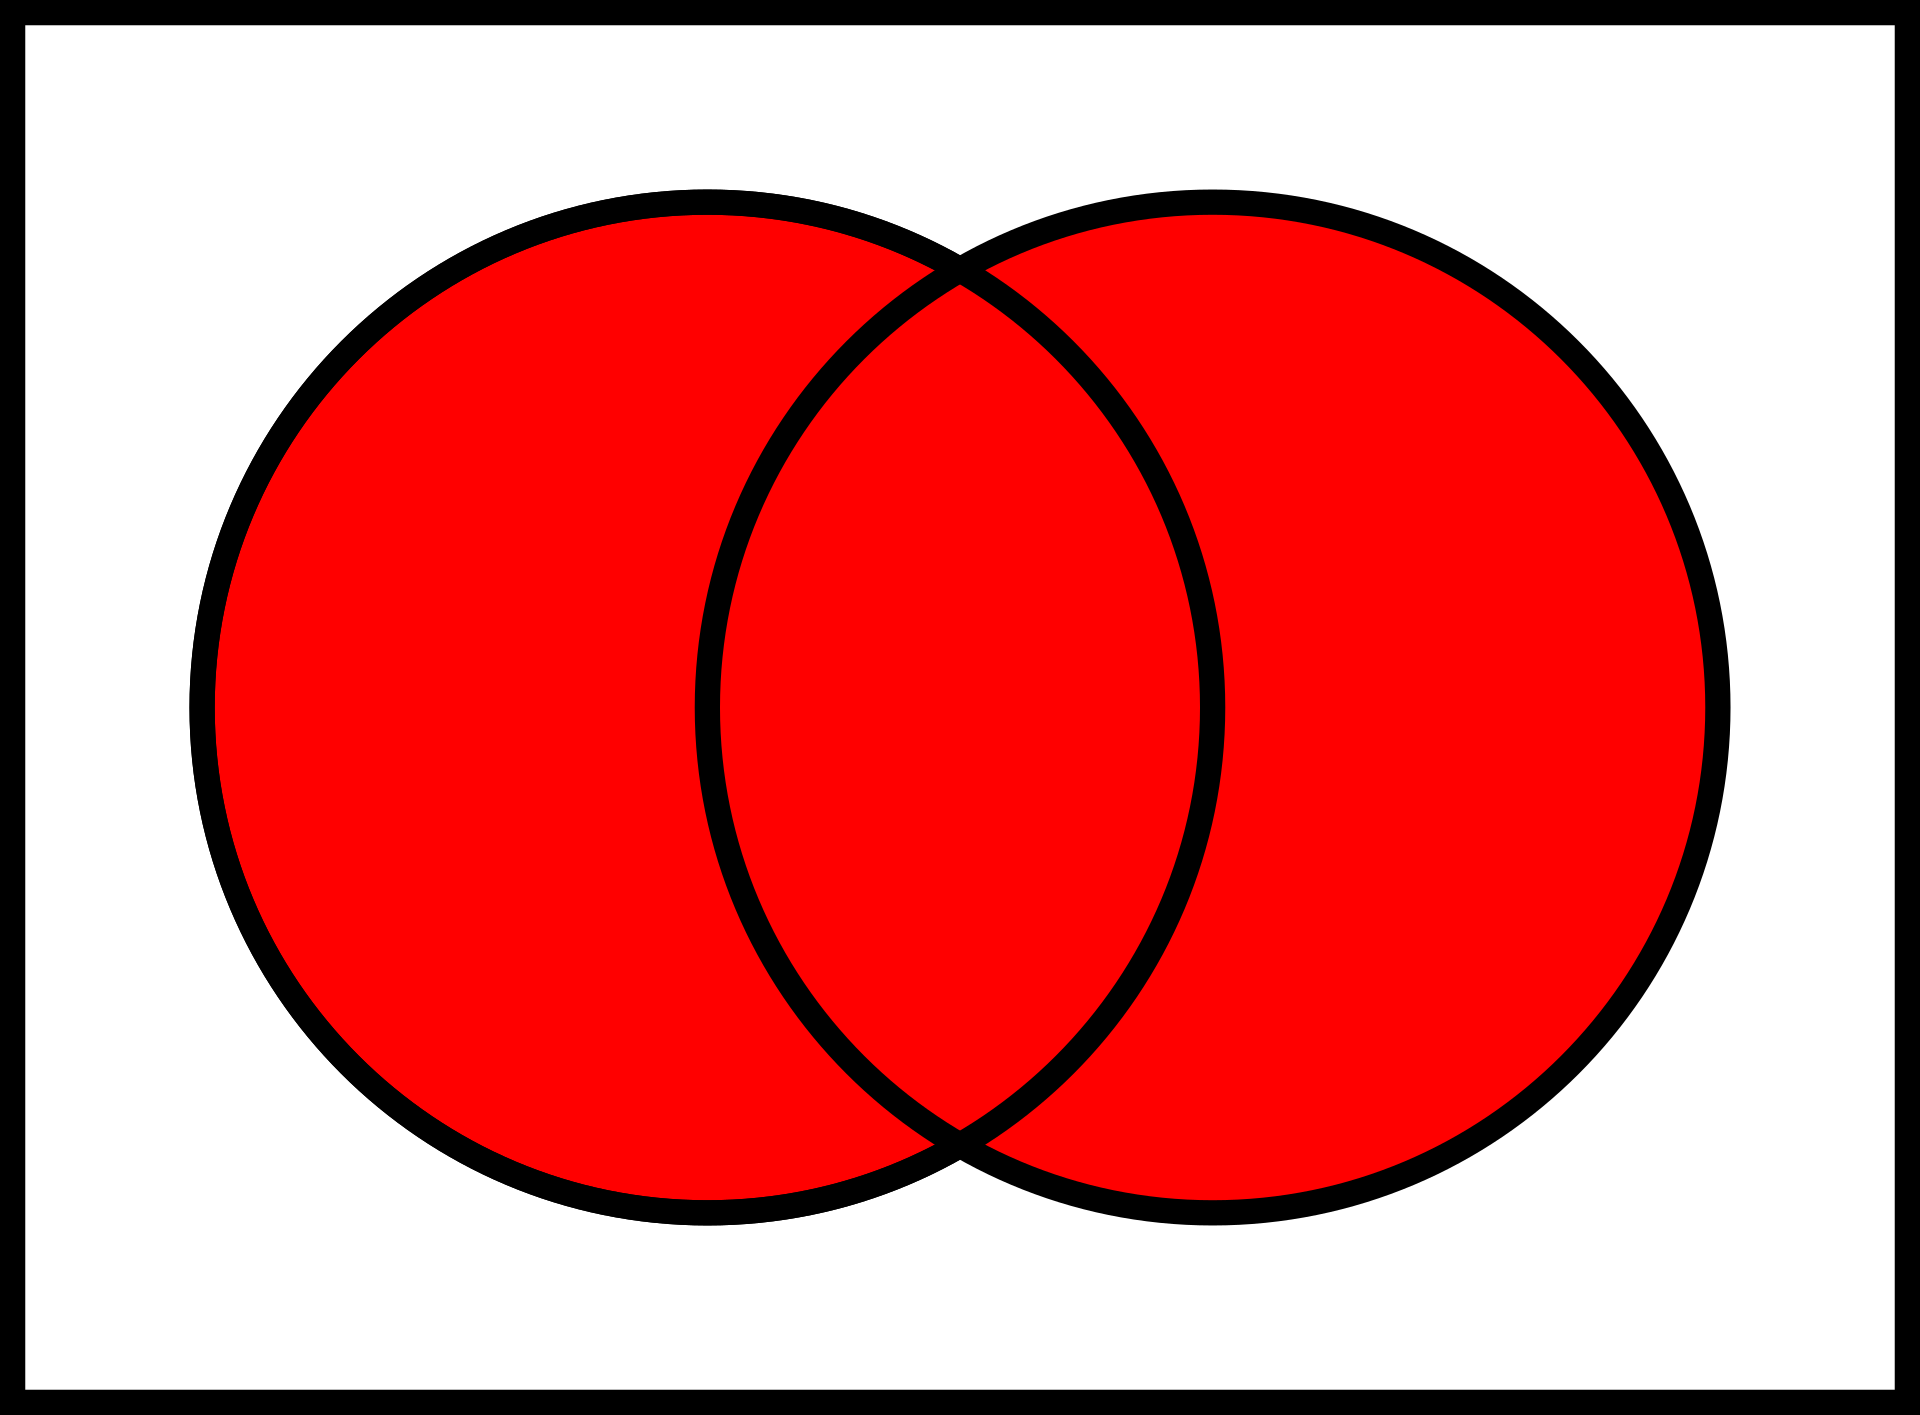
\includegraphics[width=.4\linewidth]{mehrdimWktrechnung/Venn0111.svg.png}
      \captionof*{figure}{Vereinigung \(A\cup B\)}
      \label{fig:vereinigungsmenge}
    \end{minipage}
\end{figure}

\begin{equation*}
    A\cup B = A+B-A\cap B
\end{equation*}


\subsection{Bedingte Wahrscheinlichkeit}

\begin{equation*}
    P(A|B)=\frac{P(A\cap B)}{P(B)}
\end{equation*}

\subsection{Bayes-Theorem}

\begin{equation*}
    P(A|B)=\frac{P(B|A)P(A)}{P(B)}
\end{equation*}
